\large{
Definendo la disciplina della visualizzazione delle informazioni come il mezzo per poter creare interfacce interattive per riuscire ad estrarre informazione dai dati ed avendo definito nel capitolo precedente i principi di questa particolare disciplina e alcune delle molteplici scelte applicabili è necessaria adesso una digressione sul concetto di interazione dell'utente e delle sue primitive.
\section{definizioni dell'interazione}
L'interazione assume definizioni diverse ma non discordanti tra loro a seconda dell'ambito di lavoro e del campo a cui questa fa parte. 
Per quanto concerne il campo della ricerca \textbf{HCI}, ovvero della Human Computer Interaction, l'interazione è stata definita già nel 1998 come la comunicazione tra uomo e macchina.
Per definire a pieno lo human-computer interaction e l'usabilità bisogna far riferimento al modello di Donald Arthur\textbf{ Norman}, psicologo e ingegnere statunitense. Egli identifica l'interazione utente-calcolatore nelle 7 fasi riportate di seguito: 
\begin{enumerate}
	\item formulare l'obiettivo
	\item formulare l'intenzione
	\item identificare l'azione
	\item eseguire l'azione
	\item percepire lo stato del sistema
	\item interpretare lo stato del sistema
	\item valutare il risultato rispetto all'obiettivo
\end{enumerate}
%%citare libro La caffettiera del masochista. Psicopatologia degli oggetti quotidiani (The psychology of everyday things e The design of everyday things,1988), Milano, Giunti, 1990 (ISBN 978-88-09-20182-8), 1997 (ISBN 978-88-09-21027-1), 2005 (ISBN 978-88-09-04419-7), 2009 (ISBN 978-88-09-74356-4).
Secondo \textbf{Norman} inoltre un principio fondamentale è capire gli utenti e i compiti che intendono svolgere facendo anche in modo che le interfacce utente devono consentire tali compiti nel modo più immediato e intuitivo possibile. Norman infine fa notare, nel suo libro "La caffettiera del masochista", come questo principio sia spesso inutilizzato.\\
Nel campo della ricerca nella visualizzazione delle informazioni all'interazione furono date più definizioni una successiva temporalmente alle altre. Di seguito ne sono riportate due fondamentali:
\begin{itemize}
	\item \textbf{2002} l’interazione consente la manipolazione diretta della rappresentazione grafica del dato;
	\item \textbf{2007} l’interazione fornisce agli utenti la capacità di manipolare direttamente o indirettamente e modificare le rappresentazioni.
\end{itemize}
Già da queste definizioni è possibile notare la fondamentale importanza dell'interazione dell'utente poiché una rappresentazione senza la possibilità di modifica, restando comunque utile all'utente finale, potrà solo essere analizzata staticamente in quel suo ambito di verità. Grazie all'interazione l'utente non solo potrà eseguire task di analisi ma di manipolazione creando a sua volta nuove modalità di analisi ed acquisendo consapevolezza della fondamentale importanza del fattore umano sulla macchina.

\section{classificazione}
Date le varie definizioni dell'interazione e definito il suo impiego nella visualizzazione delle informazioni è facile notare come tutte le interazioni dipendono da vari fattori che ne influenzano il comportamento e spesso anche il successo oppure il declino di un particolare sistema di visualizzazione.
Mediante i fattori visti di seguito si potrà dunque dare una classificazione dell'interazione.
\begin{itemize}
	\item \textbf{Tempo di risposta}:l'ordine di tempo a cui appartiene il tempo di risposta dell'interazione al comando dell'utente al sistema è la prima grande classificazione. Se il tempo di risposta risulta essere dell'ordine  dei $10^-1$ secondi l’interazione è velocissima e fa uso di animazioni e l'utente potrà eseguite tante operazioni in un tempo irrisorio, se risulta dell'ordine dei $10^0$ secondi l'animazione farà uso di dialoghi o finestre di dialogo che molto spesso indirizzeranno l'utente per future interazioni e se infine sarà superiore ai $10^1$ secondi interazioni saranno cognitive ovvero task che verranno eseguiti prima di ottenere risposte.
	\item \textbf{Azioni atomiche}: rispondono alla domanda "in che modo si eseguiranno le interazioni". Queste potrebbero essere eseguibili tramite tasti o azioni eseguiti con l'ausilio di un mouse o ancora potrebbero essere azioni di più alto livello come vocali, gestuali o touch.
	\item \textbf{Tecnologia}: una interazione non è nulla senza il dispositivo su cui la si esegue. Ricordando che differenti tipologie di dispositivi forniscono diversi tipi di interazioni si può classificare l'interazione anche mediante la scelta del dispositivo utilizzato che sia esso un laptops, un tablets o uno smartphone fino ad arrivare ad avere interazioni specifiche per dispositivi indossabili che riconoscono ad esempio i movimenti gestuali.
	\item \textbf{Grado di interazione}: ogni interazione possiede un grado definito come il livello di connessione e di padronanza delle operazioni che l'utente può ottenere interagendo con il sistema. In particolare il grado di interazione può essere:
	\begin{enumerate}
		\item \textbf{statico} ovvero grado $1$ in cui non è prevista alcun genere di interazione riducendo la rappresentazione ad una singola vista per una analisi non modificabile;
		\item \textbf{manipolabile} ovvero di grado $2$ in cui è possibile cambiare la vista della scena e quindi evidenziare ed analizzare meglio un dato dalla sua rappresentazione non potendo però modificare i dati da cui è nata la visualizzazione;
		\item \textbf{trasformabile} ovvero di grado $3$ dove l’interazione permette di intervenire nella fase di processo e cambiare il dato di input.
	\end{enumerate}
	\item \textbf{paradigma}: intesa come tipologia di interazione vera e propria che potrà essere tradizionale dove c’è un punto di comunicazione tra l’uomo e la macchina, realtà aumentata o la realtà virtuale.
\end{itemize}
Definite e classificate le interazioni mediante i vari fattori si può ora passare alle modalità di interazione e alle motivazioni che hanno portato a scelte utilizzate nel sistema.
\section{modalità di interazione scelte e motivazioni}
Per quanto riguarda la realizzazione del progetto essendo un editor completamente utilizzabile dall'utente sia per visualizzare che per definire strutture si è assegnato un grado di interazione pari a $3$ rendendo il sistema trasformabile per consentire all'utente in qualunque momento durante la sessione di lavoro di poter intervenire e cambiare tutto ciò che è necessario ai fini di una buona creazione e visualizzazione.
Ritornando ai tempi di risposta invece nella maggior parte delle operazioni l'utente potrà gestire interazioni con tempi dell'ordine dei $10^-1$ secondi fatta eccezione per alcune operazioni che necessariamente dovranno far uso di dialoghi introduttivi o di finestre di dialogo per poter proseguire con la visualizzazione. Lavorando con le tecnologie Web e dovendo avere un piano di lavoro di una grandezza superiore a quella di un tablet o di uno smartphone il sistema è stato pensato per poter essere utilizzato su qualunque desktop o laptop avendo quindi la possibilità di eseguire aziondi mediante l'utilizzo di bottoni cliccabili con l'ausilio di un mouse potendo quindi contare sulla velocità delle interazioni, dell'ausilio di un piano di lavoro di dimensioni considerevoli e del grado più alto di interazione si definiranno ora le \textbf{primitive} che l'utente potrà utilizzare partendo da quelle definibili basilari.\\
Le operazioni più semplici che vedremo nel dettaglio sono quelle di select con la quale l’utente seleziona un certo numero di punti da rappresentare, panning nel quale utilizza lo scrool per navigare i dati e lo zooming sia spaziale che logico.

Per quando concerne l'operazione di \textbf{select}, ricordando che un grafo clusterizzato è composto da nodi, cluster ed archi, si è scelto di dare all'utente la possibilità di selezionare e visualizzare anche solamente una dei tre insiemi di cui è composto il grafo ma senza avere la possibilità di rappresentazione di un sottoinsieme di uno di loro. È possibile quindi selezionare tutti i nodi di un grafo senza visualizzare gli archi o i cluster di cui è formato ma non è possibile selezionare esclusivamente parte di quei nodi.\\
\begin{figure}[!htb]
	\begin{center}
		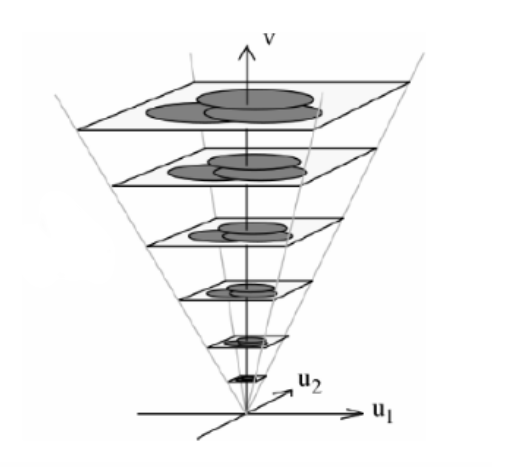
\includegraphics[width=1 \linewidth]{figure/zooming}
	\end{center}
	\caption{Operazione di zooming su un piano $<x,y>$\label{fig:zooming}}
\end{figure}
Lo \textbf{zooming} ovvero la possibilità di effettuare un ingrandimento o un ridimensionamento per potersi focalizzare su una parte spaziale di uno oggetto risulta essere una tra le principali primitive di interazione dell'utente. Lo zooming viene utilizzato per per mostrare o nascondere dati, ha significato sia spaziale che logico. E’ possibile eseguire una operazione di zooming and panning. Immaginiamo di avere un oggetto grafico disegnato su di un piano x-y ma replicato su più livelli con grado di ingrandimento diverso lungo v, come mostrato nella \figurename~\ref{fig:zooming}. La distanza dal piano x-y
determina il grado di zooming mentre il movimento sul piano x-y determina il panning.\\
Quando tengo la finestra della visualizzazione bassa riesco a includere dentro ad essa molti oggetti, man mano che si esegue lo zoom out lungo v in un punto anche diverso dal centro, per esempio dove è posizionato il puntatore del mouse, gli oggetti inclusi dalla finestra diminuiscono.
Inoltre un principio da seguire è che per muoversi lungo il piano ad un livello di zoom molto basso, ovvero quando si è lontani dall’origine e si possono vdere pochi oggetti, piuttosto che fare un panning complesso risulta più efficiente eseguire un zoom out avvicinandosi all’origine, un piccolo
panning e poi uno zoom in sino al punto di arrivo sullo stesso piano iniziale come mostrato nella \figurename~\ref{fig:panning}
\begin{figure}[!htb]
	\begin{center}
		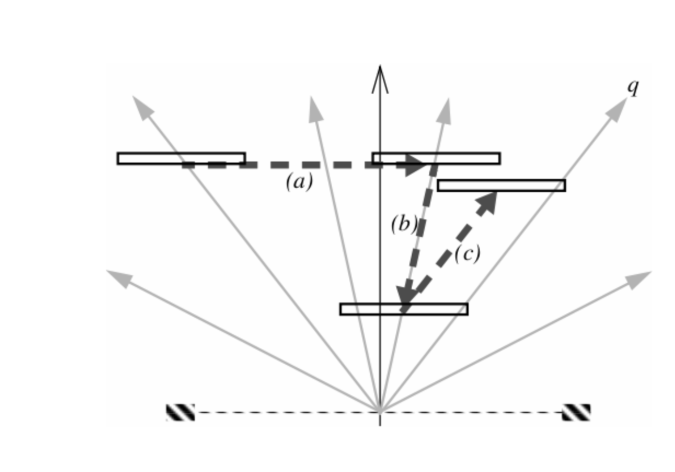
\includegraphics[width=1 \linewidth]{figure/panning}
	\end{center}
	\caption{Operazioni di panning e zooming su un piano $<x,y>$\label{fig:panning}}
\end{figure}

Per terminare con le primitive delle operazioni \textit{semplici} sarebbe necessario nominare anche il labelling ovvero l'operazione che grazie ad una interazione spesso con un tempo di risposta dell'ordine del secondo porta ad una etichettatura di un oggetto del grafo. Anche il labelling però risulta comunque una forma di zooming poiché impiegando una interazione si mostra nella rappresentazione un numero di dati più elevato come fosse uno zooming focalizzato su tutta la visualizzazione.\\
Dalle primitive di integrazione che portano alle operazioni più semplici e pressoché necessarie in ogni visualizzazione saranno ora viste nel dettaglio alcune operazioni, date comunque dall'interazione uomo-macchina con le modalità descritte prima, definibili di completezza per un sistema.
Di grande importanza infatti rappresentano la possibilità da parte dell'utente e della sua interazione di riconfigurare e di eseguire un encode dei dati.
Per quanto concerne la \textbf{riconfigurazione}, questa operazione è definita come la possibilità mediante una interazione di poter cambiare gli attributi o i dati visualizzati.E’ in questo modo possibile modificare cosa visualizzare, cambiando gli intervalli, la scala o ordinare i dati.
L'\textbf{encode }invece è definito come una modifica della visualizzazione e non dei dati. Solitamente mediante una operazione di encode si cambia il tipo di visualizzazione passando, come mostrato a titolo di esempio nella figura \figurename~\ref{fig:pieToBar}, da una rappresentazione a diagramma a barre ad una torta. Include anche operazione di modifica sui colori, sulle forme e l’orientamento della visualizzazione.
\begin{figure}[!htb]
	\begin{center}
		\hspace{-3.5 cm}
		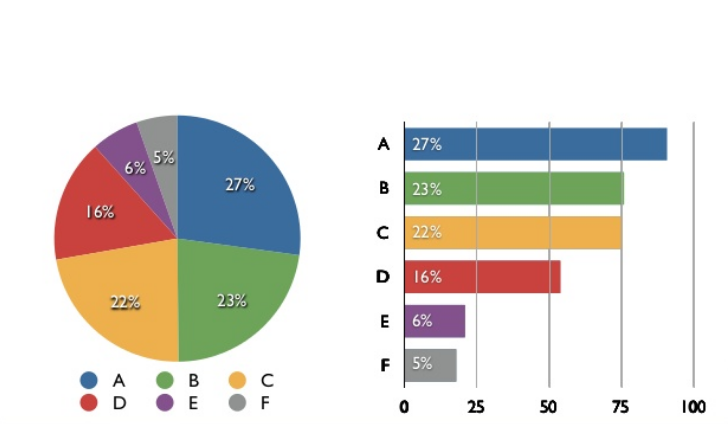
\includegraphics[width=1 \linewidth]{figure/pieToBar}
	\end{center}
	\caption{Esempio di encoding da un diagramma a torta ad uno a barre\label{fig:pieToBar}}
\end{figure}
Per quanto riguarda la realizzazione del sistema in dettaglio, la primitiva che risulta comunque essere maggiormente complessa da realizzare è però proprio quella su cui si basano le proprietà di creazione e di modifica di un oggetto facente parte del grafo: la \textbf{connessione}.
Riuscire infatti a dare all'utente la possibilità eseguire con una interazione una operazione di connessione non solo a livello grafico mediante la visualizzazione ma anche dei dati risulta essere uno degli obiettivi più complessi da raggiungere.\\
Per concludere la digressione introduttiva delle primitive di iterazione e delle operazioni eseguibili mediante le stesse e per completezza si vuol dare la definizione della primitiva di filtraggio.
Il \textbf{filtraggio} è l’operazione che permette di mostrare un sottoinsieme di dati secondo certe regole, ovvero ciò che può esser definito come uno zoom semantico. Può far uso di query tradizionali ma anche di query dinamiche. Con le query dinamiche l’operazione è rapida, immediata,cambiando un parametro la visualizzazione cambia di conseguenza, ed è immediatamente reversibile, i tempi di attesa sono minori del decimo di secondo. Nelle query classiche invece l’attesa è più alta, l’utente forma le query che vengono eseguite sulla base di un evento, che nel nostro caso risulta essere la pressione di un bottone. Tipicamente però i filtraggi eseguiti con le query dinamiche non sono complesse e le operazioni riguardano tutti i dati. È naturale pero immaginare come aumentando delle dimensioni dei dati l’interazione diviene sempre più lenta.\\ 
Il filtraggio può esser quello che, nella realizzazione del caso di studio, riguarda la possibilità di definire e differenziare i dati e le visualizzazioni dei nodi e dei cluster in quanto come visto nel capitolo relativo allo stato dell'arte presentano sostanziali differenze tra loro. 
Tutte le primitive di visualizzazione troveranno poi la loro realizzazione mediante una operazione dedicata come si vedrà nei capitoli successivi.
}
